% FlowMatchingTransformer Architecture Diagram
% Overall architecture for velocity field prediction
% Compile with: pdflatex architecture.tex
%
\documentclass[border=8pt]{standalone}
\usepackage[T1]{fontenc}
\usepackage{tikz}
\usepackage{amsmath,amssymb}
\usetikzlibrary{
    arrows.meta,
    positioning,
    calc,
    fit,
    backgrounds,
    decorations.pathreplacing
}

% ── Color Palette ──
\definecolor{inputcol}{HTML}{ECEFF1}     % Blue-gray: inputs/outputs
\definecolor{pointcol}{HTML}{80CBC4}     % Teal: point encoding
\definecolor{condcol}{HTML}{A5D6A7}      % Green: conditioning
\definecolor{concatcol}{HTML}{B39DDB}    % Lavender: concat/prepend
\definecolor{blockcol}{HTML}{EF9A9A}     % Coral: transformer blocks
\definecolor{skipcol}{HTML}{9C27B0}      % Deep purple: skip connections
\definecolor{headcol}{HTML}{FFE082}      % Amber: output head
\definecolor{normcol}{HTML}{C5E1A5}      % Light green: layer norm
\definecolor{attncol}{HTML}{FFAB91}      % Salmon: attention
\definecolor{mlpcol}{HTML}{90CAF9}       % Blue: MLP/feed-forward
\definecolor{framecol}{HTML}{757575}     % Gray: frames

\begin{document}
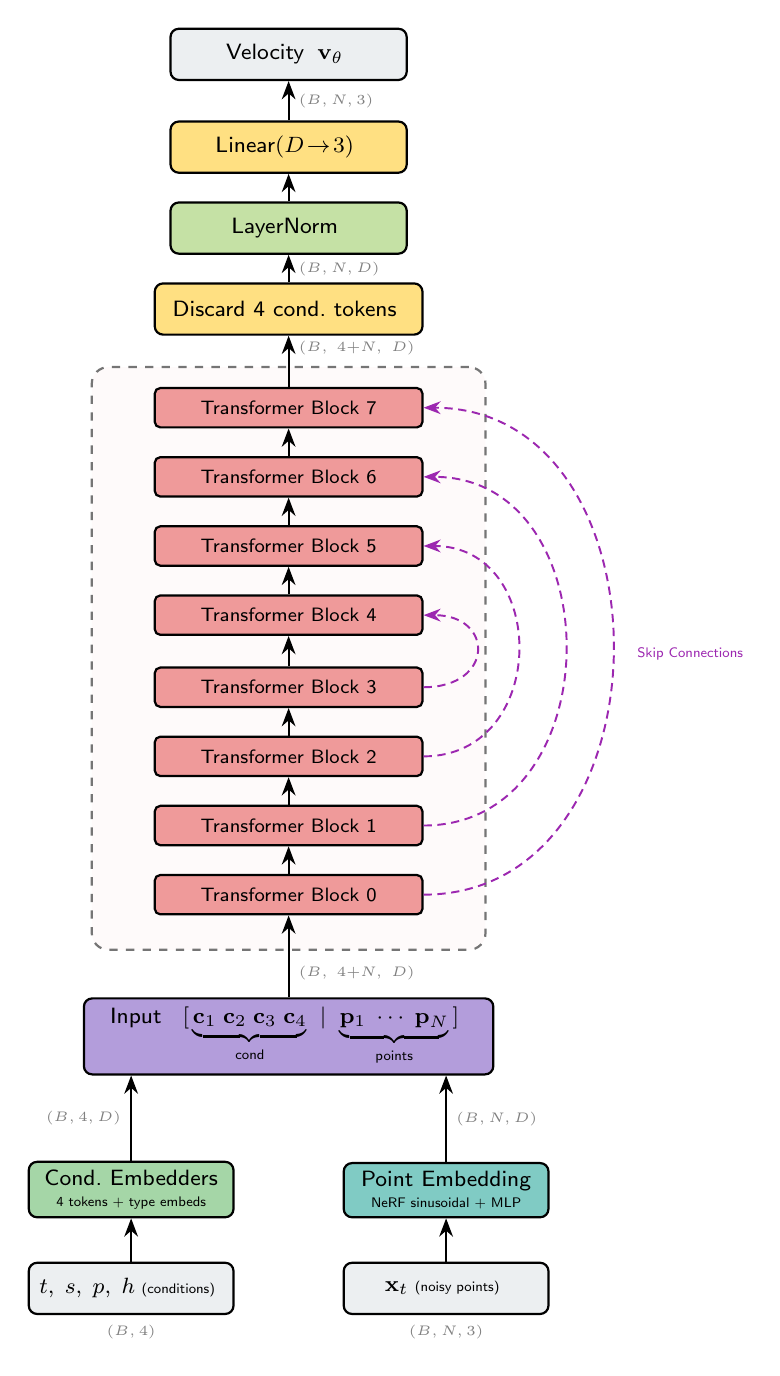
\begin{tikzpicture}[
    >=Stealth,
    font=\sffamily\footnotesize,
    % ── Node Styles ──
    mod/.style={
        draw, thick, rounded corners=3pt,
        minimum width=3.0cm, minimum height=0.65cm,
        align=center, inner sep=3pt
    },
    widemod/.style={
        draw, thick, rounded corners=3pt,
        minimum width=5.2cm, minimum height=0.65cm,
        align=center, inner sep=3pt
    },
    bmod/.style={
        draw, thick, rounded corners=2pt,
        minimum width=3.4cm, minimum height=0.50cm,
        fill=blockcol, align=center,
        font=\sffamily\scriptsize
    },
    % ── Arrow Styles ──
    arr/.style={->, >=Stealth, thick},
    skiparr/.style={->, >=Stealth, line width=0.7pt, skipcol, densely dashed},
    % ── Label Styles ──
    dl/.style={font=\sffamily\tiny, text=black!50},
    seclabel/.style={font=\sffamily\scriptsize\bfseries, text=black!40},
]

% ────────────────────────────────
%  INPUTS (y = 0)
% ────────────────────────────────
\node[mod, fill=inputcol, minimum width=2.6cm] (ci) at (-2.0, 0) {
    $t,\; s,\; p,\; h$\;{\tiny(conditions)}
};
\node[dl] at (-2.0, -0.55) {$(B, 4)$};

\node[mod, fill=inputcol, minimum width=2.6cm] (xt) at (2.0, 0) {
    $\mathbf{x}_t$\;{\tiny(noisy points)}
};
\node[dl] at (2.0, -0.55) {$(B, N, 3)$};

% ────────────────────────────────
%  EMBEDDINGS (y ≈ 1.5)
% ────────────────────────────────
\node[mod, fill=condcol, minimum width=2.6cm, above=0.55cm of ci] (ce) {
    Cond.\ Embedders\\[-2pt]
    {\tiny 4 tokens + type embeds}
};

\node[mod, fill=pointcol, minimum width=2.6cm, above=0.55cm of xt] (pe) {
    Point Embedding\\[-2pt]
    {\tiny NeRF sinusoidal + MLP}
};

\draw[arr] (ci) -- (ce);
\draw[arr] (xt) -- (pe);

% ────────────────────────────────
%  INPUT SEQUENCE (y ≈ 3.2)
% ────────────────────────────────
\node[widemod, fill=concatcol] (prep) at (0, 3.2) {
    Input\;\;
    $[\,\underbrace{\mathbf{c}_1\;\mathbf{c}_2\;\mathbf{c}_3\;\mathbf{c}_4}_{
        \text{\tiny cond}}\;
    \mid\;
    \underbrace{\mathbf{p}_1 \;\cdots\; \mathbf{p}_N}_{\text{\tiny points}}\,]$
};

% Arrows from embeddings to input sequence with dimension labels
\draw[arr] (ce.north) -- (ce.north |- prep.south)
    node[midway, left, dl] {$(B, 4, D)$};
\draw[arr] (pe.north) -- (pe.north |- prep.south)
    node[midway, right, dl] {$(B, N, D)$};

% ────────────────────────────────
%  TRANSFORMER BACKBONE
% ────────────────────────────────

% Background frame
\begin{scope}[on background layer]
    \node[draw, thick, rounded corners=6pt, dashed,
          color=framecol, fill=blockcol!5,
          minimum width=5.0cm, minimum height=7.4cm]
          (uvit_frame) at (0, 8.0) {};
\end{scope}

% ── Blocks 0–3 ──
\node[bmod] (B0) at (0, 5.0) {Transformer Block 0};
\node[bmod, above=0.35cm of B0] (B1) {Transformer Block 1};
\node[bmod, above=0.35cm of B1] (B2) {Transformer Block 2};
\node[bmod, above=0.35cm of B2] (B3) {Transformer Block 3};

% ── Blocks 4–7 ──
\node[bmod] (B4) at (0, 8.55) {Transformer Block 4};
\node[bmod, above=0.35cm of B4] (B5) {Transformer Block 5};
\node[bmod, above=0.35cm of B5] (B6) {Transformer Block 6};
\node[bmod, above=0.35cm of B6] (B7) {Transformer Block 7};

% ── Sequential flow arrows ──
\draw[arr] (prep) -- (B0)
    node[pos=0.3, right, dl] {$(B,\; 4{+}N,\; D)$};
\draw[arr] (B0) -- (B1);
\draw[arr] (B1) -- (B2);
\draw[arr] (B2) -- (B3);
\draw[arr] (B3) -- (B4);
\draw[arr] (B4) -- (B5);
\draw[arr] (B5) -- (B6);
\draw[arr] (B6) -- (B7);

% ── Skip Connections (right side arcs) ──
\draw[skiparr]
    (B0.east) .. controls +(3.2, 0) and +(3.2, 0) .. (B7.east);
\draw[skiparr]
    (B1.east) .. controls +(2.4, 0) and +(2.4, 0) .. (B6.east);
\draw[skiparr]
    (B2.east) .. controls +(1.6, 0) and +(1.6, 0) .. (B5.east);
\draw[skiparr]
    (B3.east) .. controls +(0.9, 0) and +(0.9, 0) .. (B4.east);

% Skip connection label
\node[font=\sffamily\tiny, text=skipcol, align=center]
    at (5.1, 8.05) {Skip Connections};

% ────────────────────────────────
%  OUTPUT SECTION
% ────────────────────────────────
\node[mod, fill=headcol, minimum width=3.4cm, above=0.65cm of B7] (slice) {
    Discard 4 cond.\ tokens
};

\node[mod, fill=normcol, minimum width=3.0cm, above=0.35cm of slice] (lnorm) {
    LayerNorm
};

\node[mod, fill=headcol, minimum width=3.0cm, above=0.35cm of lnorm] (linout) {
    Linear$(D \!\to\! 3)$
};

\node[mod, fill=inputcol, minimum width=3.0cm, above=0.50cm of linout] (vel) {
    Velocity\;\;$\mathbf{v}_\theta$
};

% Output arrows with dimension labels
\draw[arr] (B7) -- (slice)
    node[pos=0.75, right, dl] {$(B,\; 4{+}N,\; D)$};
\draw[arr] (slice) -- (lnorm)
    node[midway, right, dl] {$(B, N, D)$};
\draw[arr] (lnorm) -- (linout);
\draw[arr] (linout) -- (vel)
    node[midway, right, dl] {$(B, N, 3)$};

\end{tikzpicture}
\end{document}
